\section{Dokumentation}

I dette afsnitt er projektets filer, funktioner, moduler og makroer dokumenteret og beskrevet. Fokuset er på funktionernes vigtigste egenskaber og virkemåder. Filerne med tilhørende funktioner er delt op i tre forskellige lag: Application, Application Interface og Hardware Abstraction Layer. Se figur \ref{block}.
 I Application Layer ligger de applikationspecifikke filer, disse filer kan bruges på anden hardware uden at modificere dem. I Hardware Abstraction Layer ligger de hardwarespecifikke filer. Disse filer muligør kommunikation mellem hardware og vores software. Disse filer kan benyttes i helt andre programmer såfremt det er samme type hardware der benyttes. 

\begin{figure}[h]
\begin{center}
\label{block}
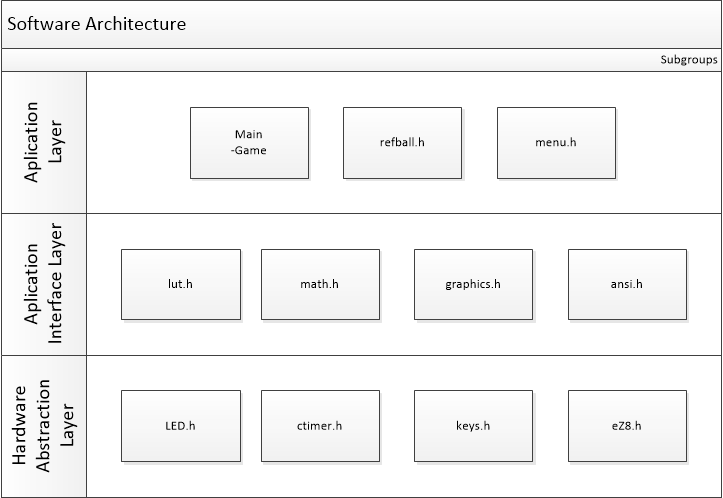
\includegraphics[scale=0.6]{img/SoftwareArchitecture.png}
\caption{Block diagram over de forskellige lag}
\end{center}
\end{figure}
\textit{\textbf{Vi har udviklet alle moduler i fællesskab, og det giver ikke mening at tilskrive nogle personer en særlig del af koden, da meget lidt kode er skrevet af udelukkende en person.} }
\newpage
\subsection{Application layer}
I dette lag findes refball modulet, menu modulet og main modulet.
\subsubsection{main.c}
ReflexBall styres af \textbf{main.c} som består af to funktioner. \textbf{Main} styrer den overordnede kørsel av programmet og menuen, og \textbf{Game} kontrollerer de forskellige levels og selve gameplayet. Se nærmere beskrivelse af \textbf{main.c} under implementation.

\subsubsection{refball.h}
refball.h er et modul der indeholder grundlæggende regler om spillet: kollision, hvordan bolden skal bevæge sig og hvorledes strikeren skal opføre sig. Desuden indeholder den strukturerne \textit{Ball} og \textit{Box}. Ydermere indeholder dette modul også særligt mange konstanter.
\paragraph{Strukturen Ball}
\textit{Ball} er en stuktur som har variablene opgivet i \ref{Ballkrav}. \textit{outOfBounds}, der fortæller om spilleren er inde for banen, og \textit{powerActivated}, der fortæller om high power er aktiveret, er implementeret som unsigned char's. I \textit{power}, gemmes hvor meget power spilleren har opladet.
 

\paragraph{Strukturen Box}
\textit{Box} er en struktur der indeholder samtlige bokse i spillet. Den indeholder 3 pointere til char-arrays: et koordinatsæt og et tilhørende array med boksenes styrke. Desuden er der to variable der fortæller antallet af bokse der er fyldt i stacket og hvor mange der ikke er ødelagte. I designfasen forestillede vi os at den skulle implementeres som et stack, således arrayernes størrelse var variable, men hvorfor vi ikke gjorde det står i afsnit \ref{reallocfejl}.
\paragraph{void moveBall(Ball * ball)}
Denne funktion flytter bolden ved at tage en peger til en \textit{Ball} som argument og lægger retningsvektoren til x og y koordinaterne.
\paragraph{void moveStriker(long * x,char direction)}
Denne funktion tager to variable som argumenter, en pointer til strikerens x-lokation, og  strikerens retning. Hvis \textit{direction} er 1 bevæger strikeren sig mod positiv x-retning og STRIKER\_SPEED lægges til, ellers bevæger strikeren sig mod negativ x-retning og STRIKER\_SPEED fratrækkes strikerens x-lokation.
\paragraph{unsigned char checkBall(Ball * ball,Box * box,  int x)}\
checkBall() er en funktion som kontrollerer og bestemmer boldens bevægelse. checkBall tager bolden, kasserne og strikerens position som argumenter. I funktionen gennemgåes de forskellige scenarier, hvor bolden kan ramme. Først kontrolleres om strikeren er ramt, derefter om kanterne er ramt og til sidst gennemgås alle kasserne og kontrolleres for om de er ramt. Hvis kassen bliver ramt ændres der i boldens retningsvektor, alt afhængigt af hvordan kassen rammes. Endeligt returnerer funktionen et tegn, svarerende til det, bolden har ramt. Hvis bolden intet har ramt foretages ingen ændring på retningsvektorerne, og et blankt tegn sendes tilbage. 
\paragraph{long toTerminalCoordinates(long x)}\
Denne funktion omdanner tal i 2.14 eller 18.14 til heltal man kan bruge i terminalen. Afrunding laves som vanligvis, ved at afrunde til nærmeste heltal.

\paragraph{void setBallOverStriker( Ball * ball, long st)}
Denne funktion sætter bolden over strikeren.
Funktionen omdanner st til 18.14 format og sætter boldens x-koordinat til dens værdi.
Boldens y-koordinat sættes over strikeren, vha. konstanterne STRIKER\_Y og OVER\_STRIKER, også i 18.14. Boldens retningsvektor sættes derefter til at gå lodret op, og roteres derefter 40 grader mod venstre.
\paragraph{Box * newBoxStack()}
Denne funktion bliver brugt til at lave et nyt \textit{Box}-stack. Der bliver allokeret plads, så der er plads til antallet af bokse givet ved konstanten MAX\_BOXES. Antallet af elementer, \textit{size}, i stacket sættes til 0 og  pegeren til \textit{Box}-stacket.
\paragraph{
void createBoxes( Box * box,char level)}\
Denne funktion tager en peger til Box-stacket og en character der repræsenterer level som argumenter.  Afhængigt af levels værdi, bliver Box-stacket fyldt på en speciel måde, således hvert level er unikt. 

\subsubsection{menu}
Dette modul indeholder funktioner til at tegne og vise grafik når man bevæger sig rundt i menuen.
\paragraph{void initiateMenu()}\
Denne funktion renser først skærmen og printer derefter menuen. Slutteligt sættes markøren på Start Game.
\paragraph{void moveMarker(int selectedOption)}\
Denne funktion sætter markøren alt afhængigt af inputtet.
\paragraph{void printDifficulty(short diff)}\
Denne funktion har til formål at printe sværhedsgraden når brugeren vælger:
\begin{enumerate}
\item Hvis \textit{diff} er 1, skrives der "Easy"
\item Hvis \textit{diff} er 2, skrives der "Normal"
\item Hvis \textit{diff} er 3, skrives der "Hard"
\end{enumerate}
\paragraph{void printHelp()}
Denne funktion printer hjælpe-teksten. Startstedet for teksternes x-koordinat bestemmes af konstanten LEFT\_BORDER

\subsection{Application Interface Layer}
\subsubsection{graphics.h}
Dette modul indeholder grafiske elementer til brug i terminalen. Nogle af funktionerne er særligt udviklet til dette spil, men det er muligt de også ville kunne bruges i andre sammenhæng.  Det kan derfor diskuteres om funktionen strengt taget liger i API-laget. Måske den kan siges at ligge i grænsefeltet.
\paragraph{
void drawBox(unsigned char x, unsigned char y,unsigned char color)}\
Denne funktion tegner en boks med bredden givet ved argumentet og højden 2. Koordinaterne til det øverste venstre hjørne gives som argumenter, sammen med kassens farve, hvor farveskemaet i fgcolor bruges.

\paragraph{void drawChar(unsigned char x, unsigned char y,char tegn)}\
Denne funktion tager et koordinatsæt og et tegn som argumenter. Tegnet bliver skrevet på det givne koordinatsæt.

\paragraph{void moveDrawStriker(unsigned char x, unsigned char direction)}\
heeej

\paragraph{void drawBounds(int x1,int y1, int x2, int y2,unsigned char color)}\
Denne funktion tegner banens kanter. Den tager 2 koordinatsæt som input, x1 og y1 svarende til det øverste venstre hjørne og  x2 og y2 svarende til det nederste højre hjørne. Variablen color bruges til at bestemme farven på kanterne. 

\paragraph{void drawLogo()}\
Denne funktion tegner spillets logo. Den bruger konstanten LEFT\_BORDER til at bestemme på hvilket x-koordinat den skal begynde at skrive fra, således det bliver logoets venstre kant.
\paragraph{drawBall(unsigned char x, unsigned char y, unsigned char color)}
Denne funktion tager et koordinatsæt og printer et o i farven bestemt af det 3. parameter.

\paragraph{void drawStriker(unsigned char x, unsigned char color, char strikerWidth, char strikerY)}
Denne funktion tegner blot en striker centrummet for strikeren er x, color er farven, strikerWidth er bredden på hver side, og strikerY er Y-koordinatet.

\paragraph{void drawGameOver()}
Denne funktion tegner ASCII-kunst af /textit{GAME OVER} og scroller den ud af skærmen.

\paragraph{void drawVictory()}
Denne funktion tegner ASCII-kunst af Arnold Schwarzenegger og scroller den ud af skærmen.

\paragraph{void scrollText(char y, char delay)}
Denne funktion printer mange linjer med mellemrum sådan at det der tidligere er skrevet bliver scrollet væk.

\paragraph{void printExampleBoxes(char x, char y, char boxSize)}
Denne funktion printer de 5 typer bokser der bruges i spillet sådan at brugeren kan se hvor meget de forskellige boksr tåler.

\subsubsection{lut.h}
\label{lut}
Dette modul indeholder en konstant tabel med sinus værdier for en cirkel delt i 512 stykker. Hvis x er vinklen i radian indsættes da blot $\dfrac{x\cdot \pi}{256}$ i tabellen.
\subsubsection{math.h}
Dette modul indeholder nogle generelle matematiske funktioner, heriblandt sin og cosinus, og to makroer til at regne i 2.14 eller 18.14.
\paragraph{Makroer}\
Modulet indeholder to makroer, en til at multiplicere to tal i .14 format, og en til at dividere to tal i .14 format, hhv. FIX14\_MULT(a, b) og FIX14\_div(a,b)

\paragraph{(void rotate(Ball * ball , int ang)}
Denne funktion tager en peger til en Ball og en int som argument. Den rotererer derefter bolden med værdien af intgeren givet i argumentet.

\paragraph{long sin(int x)}\
Denne funktion tager en int som argument. Vinklen skal ikke være i radian, men skal bruge opdelingen af cirklen beskrevet i afsnit \ref{lut}. Der returneres sinus til den givne vinkel.
\paragraph{long cos(int x)}\
Denne funktion tager en int som argument. Vinklen skal ikke være i radian, men skal bruge opdelingen af cirklen beskrevet i afsnit \ref{lut}. Der returneres cosinus til den givne vinkel.
\subsection{Hardware Abstraction Layer}
\subsubsection{keys.h}
Dette modul får inputs fra knapperne, og kan debounce ved hjælp af timer.h

\paragraph{char readKey()}
Denne funktion læser fra knapperne, og returnerer en bit streng, hvor de tre knapper er på hver deres plads i strengen. Hvis pladsen tilhørende knappen er 1, betyder det at knappen bliver trykket. Denne funktion kan godt detektere hvis brugeren trykker flere knapper ind samtidigt. Pladserne er konfigureret således:
\begin{enumerate}
\item Knappen til højre er på LSB(least significant bit)
\item Den midterste knap er på 1. plads i bit-strengen.
\item Knappen til venstre er på 2. plads i bit-strengen.
\end{enumerate}

\paragraph{char getKey()}\
Denne funktion bruges hvis man ønsker debouncing. Den læser vha. readKey() og checker derefter om værdien er det samme efter 10 ms og returner dette.
\subsubsection{ctimer.h}
Dette modul har med vores primære timer at gøre. Den har 2 globale variable: \textit{time} og \textit{timeWait}. Time tæller hvor lang tid timeren har været tændt. Grunden til at vi har globable variable her, er fordi timeren skal være uafhængig af main og køre så hurtigt som muligt. Main funktionen kan få adgang til variablene ved nogle setter- og getter-funktioner
\paragraph{void setTimer()}\
Denne funktion sætter vores timer til prescaling 0, continous mode og høj prioritet for interrupt funktionen. Denne timer er sat til at køre hvert ms.
\paragraph{void resetTimer()}\
Denne funktion sætter de til modulet tilhørende globale variable, \textit{time} og \textit{timeWait}, til 0.
\paragraph{void timer0int}\
Dette er interruptfunktionen tilhørende timeren. Den lægger 1 til \textit{time} og trækker 1 fra \textit{timeWait}. 
\paragraph{void SetDelay(int input)}\
Denne funktion sætter timeWait til værdien givet i argumentet. Meningen er at bruge \textit{timeWait} som en slags delay, man kan checke værdien på
\paragraph{int getDelay}\
Denne funktion er blot en getter, der returnerer \textit{timeWait}
\paragraph{unsigned long getCentis()}\
Denne funktion er blot en getter, der returnerer \textit{time}
\subsubsection{LED.h}
I dette modul bruges der nogle globale variable. Dette gøres for at f.eks. kunne holde styr på hvilken kolonne og LED-enhet der skal lyse. Det hadde været muligt at undgått brugen af globale variable, men da ville man være nødt til at sende mange flere variable som parametre fra main. Dette ville ikke øge effektiviteten af programmet, men snarere gjort det hele mere kompliceret eftersom dette modul kører på sin egen frekvens. Og siden variablene kun er relevante for modulet er det ikke nogen idé i at de ligger i main.

\paragraph{void LEDInit()}
Denne funktion indstiller TIMER1 til at give et interrupt hvert 0.5 ms. Envidere initialiseres de globale variabler i LED.C.

\paragraph{void timer1int()}
Denne funktion kaldes af interrupts fra TIMER1 på boardet. Denne funktion kalder funktionen LEDUpdate().

\paragraph{void setLedMode(char valueIn)}
Denne funktion er blot en setter der kontrollerer hvilken funktion der kaldes af LEDUpdate.

\paragraph{void LEDUpdate()}
Denne funktion kalder en af to funktioner, LEDUpdateOnce() eller LEDUpdatePrint().

\paragraph{void LEDSetString(char *string)}
Denne funktion læser en streng  og kopierer den over til den globale variabel /textit{string}. Envidere nulstiller den de globale variable.

\paragraph{void LEDLoadBuffer()}
Denne funktion indlæser bufferen fra et karakterset på den måde, at når funktionen LEDUpdatePrint() kaldes er teksten umiddelbart på displayet. Med andre ord; denne funktion gør at teksten ikke ruller ind og er derfor nyttig når man skal opdatere displayet hurtigt.

\paragraph{void LEDUpdatePrint()}
Denne funktion bruger tids-multiplexing til at belyse alle kolonnene. For at få dette til at fungere bruges to variable der holder styr på hvilken LED-enhed og kolonne der skal lyse.

\paragraph{void LEDUpdateOnce()}
Denne funktion ruller en tekststreng over displayet og holder på de sidste fire tegn. Displayet multiplexes på samme måde som i LEDUpdatePrint(), men strengen bliver også rullet. For at kontrollere hastigheden bruges en tæller.



